\documentclass[conference]{IEEEtran}

\usepackage{cite}
\usepackage{pslatex} % -- times instead of computer modern, especially for the plain article class
\usepackage[colorlinks=false,bookmarks=false]{hyperref}
\usepackage{booktabs}
\usepackage{graphicx}
\usepackage{xcolor}
\usepackage{multirow}
\usepackage{comment}
%\usepackage{flushend} % even out the last page, but use only at the end when there is a bibliography

\newcommand{\code}[1]{{\small{\texttt{#1}}}}

% fatter TT font
\renewcommand*\ttdefault{txtt}
% another TT, suggested by Alex
% \usepackage{inconsolata}
% \usepackage[T1]{fontenc} % needed as well?

\usepackage{listings}

%\newcommand{\todo}[1]{{\emph{TODO: #1}}}
\newcommand{\todo}[1]{{\color{olive} TODO: #1}}
\newcommand{\martin}[1]{{\color{blue} Martin: #1}}
\newcommand{\andrew}[1]{{\color{red} Andrew: #1}}
\newcommand{\tjark}[1]{{\color{orange} Tjark: #1}}
\newcommand{\rewrite}[1]{{\color{red} rewrite: #1}}

% uncomment following for final submission
%\renewcommand{\todo}[1]{}
%\renewcommand{\martin}[1]{}


%%Uncomment the following when you want to add copyright notice and not use any space	 (IEEE only)
%\usepackage[absolute]{textpos}
%% Set unit to be pagewidth and height, and increase inner margin of box
%\setlength{\TPHorizModule}{\paperwidth}\setlength{\TPVertModule}{\paperheight}
%\TPMargin{5pt}
%% Define \copyrightstatement command for easier use
%\newcommand{\copyrightstatement}{
%	\begin{textblock}{0.85}(0.072,0.93)    % Tweak here: {box width}(leftposition, rightposition)
%		\noindent
%		\normalsize
%		???-?-?-???-?/??/\$31.00~\copyright20?? IEEE % Put here your copyright
%	\end{textblock}
%}

\begin{document}


%\title{Towards Verification of Digital Circuits with\\
%SystemVerilog/UVM and Chisel/Scala}

\title{Functional Coverage-Driven Fuzzing for Chisel Designs}

\author{


\IEEEauthorblockN{Andrew Dobis, Tjark Petersen, Martin Schoeberl}
\IEEEauthorblockA{\textit{Department of Applied Mathematics and Computer Science} \\
\textit{Technical University of Denmark}\\
Lyngby, Denmark \\
adobis@student.ethz.ch, s186083@student.dtu.dk, masca@dtu.dk}
}


\maketitle \thispagestyle{empty}

\begin{abstract}

Verification of Digital Systems must be done in ever tighter time constraints due to the rise of domain-specific hardware accelerators.
To combat this, we must learn from agile techniques used software engineers and bring them to the hardware realm.
In this mindset, Chisel, a hardware construction language embedded in Scala, was developed as a tool to accelerate the implementation of digital designs.
Following this path, we developed a high level verification library named ChiselVerify, bringing tools such as Functional Coverage to the Chisel ecosystem.
Using this tool, we propose a functional coverage-driven mutation-based fuzzer for Chisel designs.
Experiments on the Leros accumulator ALU show that the additional dut information inherent in functional coverage enables the fuzzer to attain a target coverage percentage in less iterations than when using branch coverage.

\end{abstract}

\begin{IEEEkeywords}
digital design, verification, fuzzing, coverage
\end{IEEEkeywords}
%\martin{We aim for \url{https://woset-workshop.github.io/WOSET2020.html}}
%\section{TODO}
%
%Ref our last WOSET paper
%
%\todo{Rewrite all what is left over now, as this is a copy of the last WOSET paper and from the verify paper}
\section{Introduction}
\label{sec:intro}

In recent years, we have seen an increase in the demands for high performance computing systems.  
This comes with an increase in the need for domain-specific hardware accelerators.  
Designing these is time-consuming and error prone, which is why researchers have been focusing on increasing the efficiency of Hardware Verification tools to fight this added time constraint.
This has lead to the introduction of verifications methods, such as constrained random verification and functional coverage~\cite{verify:chisel:2020, dobis2021opensource}, into high level hardware construction languages, like the Scala-embedded language Chisel~\cite{chisel:dac2012, chisel:book} .
These tools, inspired by the more hardware-centric approach given in SystemVerilog and UVM, enable basic verification, where the user has to handle the writing of all tests by hand.
To improve the efficiency of these tools, we propose a form of dynamic verification, based on coverage-driven mutation-based fuzzing techniques found in the Software world.
This allows for optimal fuzzing for RTL designs using functional coverage as a metric to drive the fuzzing.

This paper describes a research project that aims to develop an optimal functional coverage-driven mutation-based fuzzing tool to test RTL circuits.
We plan on building upon this tool to enable constrained random program generation allowing for fuzzing to be used to test processors.

This paper is organized in six sections: % The following section presents related work.
Section~\ref{sec:related}  Presents related work.
Section~\ref{sec:tools} describes the open-source tools that we use in our project.
Section~\ref{xxx} presents our open-source fuzzing library, which is part of ChiselVerify.
Section~\ref{sec:eval} evaluates our approach with a small design example written in Chisel, VHDL,
and Verilog.
Section~\ref{sec:conclusion} concludes.


%\rewrite{Recent advances with SystemVerilog and Chisel \cite{chisel:dac2012, chisel:book} have brought object-oriented programming
%into the digital design and verification process. SystemVerilog, an extension of Verilog, adds object-oriented concepts for the non synthesizable verification code.
%Chisel is a ``Hardware Construction Language'', embedded in Scala, to describe digital circuits.
%Circuits described in Chisel can be tested and verified with a Chisel testing framework and Scala tests.
%Scala/Chisel brings object-oriented and functional programming into the world of
%digital design.
%
%
%This paper describes a research project that aims to build a testing framework in Scala
%that takes the best methods from the Universal Verification Methodology (UVM) and
%decades of experience in software testing.
%Furthermore, we aim to build on open-source projects only. Therefore, our
%work is open-source as well.
%
%The main contribution of this paper is
%
%This paper is organized in six sections: % The following section presents related work.
%Section~\ref{sec:related}  Presents related work.
%Section~\ref{sec:tools} describes the open-source tools that we use in our project.
%Section~\ref{xxx} presents our open-source fuzzing library, which is part of ChiselVerify.
%Section~\ref{sec:eval} evaluates our approach with a small design example written in Chisel, VHDL,
%and Verilog.
%Section~\ref{sec:conclusion} concludes.}
%


\section{Related Work}
\label{sec:related}
We will now present work related to current developments in hardware verification and fuzzing for RTL circuits.
%
%\martin{What does SV and UVM bring on the table related to fuzzing? Someone must have tried it.}
%\andrew{Fuzzing is a very software thing to do, it's only been noticed by verification engineers in recent years, the only "completed" work I've found on fuzzing for hardware is Kevin's stuff. Everything else is very conceptual and not complete.}

The Universal Verification Methodology (UVM) is a methodology for testing and verifying of digital circuits.
UVM is implemented as a SystemVerilog library and utilizes the fact that SystemVerilog uses object-oriented programming when designing testbenches.
Using object-oriented patterns such as inheritance and polymorphism, the verification engineer can design generic components that can be extended and modified to provide application-specific functionality.
As of 2017, it has been standardized as IEEE 1800.2~\cite{IEEE:18002}.
UVM is a first step towards truly standardized test-benches.

At the time of writing, very little published work was done in the realm of fuzzing for RTL circuits.
One project, named RFuzz~\cite{rfuzz2018} and lead by researchers at UC Berkeley, focuses on ``coverage-guided fuzz mutational testing''. This method relies on FPGA-accelerated simulation and new solutions allowing for quick and deterministic memory resetting, to efficiently use fuzzing on RTL circuits. The coverage metrics used in this solution are automated and based on branch coverage. RFuzz is currently no longer in development (last commit is from July 2020). This work differs from what we present in this paper in two ways. First, RFuzz uses a very simple coverage metric that is independent of the DUT (Device Under Test), while we guide our fuzzing using functional coverage, which inherently contains information about the DUT. Functional coverage is obtained using tools from ChiselVerify~\cite{verify:chisel:2020, dobis2021opensource}. Another difference is in the randomized program generation, while RFuzz only generates random bit streams, our goal is to focus as well on the generation of coherent random programs, allowing one to test a processor more efficiently. 

An other important project in the realm of fuzzing is AFL (American Fuzzy Lop)~\cite{afl:repo}, which is a statement coverage driven fuzzer for software developed by researchers at Google. AFL is similar in many ways to RFuzz and to our solution, since it is also a mutation-based fuzzer. However, the main difference is obvious, AFL is a fuzzer for software, while the two other fuzzers are for RTL circuits. This doesn't change the fact that many of the internals of our are similar to those of AFL.

As far as we know, our solution, which is part of the verification library ChiselVerify, is the only mutation-based fuzzer for RTL circuits that uses functional coverage to drive the test generation.

%\rewrite{Other projects have also focused on applying software testing techniques to hardware verification. RFuzz~\cite{rfuzz2018} focuses on creating a generalized method that enables efficient ``coverage-guided fuzz mutational testing''. This method relies on FPGA-accelerated simulation and new solutions allowing for quick and deterministic memory resetting, to efficiently use fuzzing (i.e. randomized testing, where the random seeds are updated depending on certain coverage results) on RTL circuits. The coverage metrics used in this solution are automated and based on branch coverage. This work offers a different type of solution. While we work mostly on verification functionalities inside a language, RFuzz delivers an efficient way to use said functionalities in order to ameliorate testing. RFuzz uses functional coverage tools in order to guide its randomized testing. A similar result could be obtained by combining the Constrained Random Verification and Functional Coverage tools that are available in ChiselVerify.

%\texttt{Chisel3.formal}  is a formal verification package containing a set of tools and helpers for formally verifying Chisel modules~\cite{chisel:formal}. The approach taken here is quite different from what we have developed. Rather than creating a set of tools that supplement the current chisel testing pipeline, \texttt{chisel3.formal} rather proposes a different way of testing, based around defining a set of formal checks that a design must pass in order to be considered as functional. These checks can, for example, look like: \texttt{past(io.out, 1) (pastIoOut => \{ assert(io.out >= pastIoOut) \})} which guarantees that the current module will never decrease its output from one cycle to the next. These formal checks can then be verified by calling the \texttt{verify(module)} function. 
%
%This approach is similar to software contracts in Scala. The main difference between our solution and this one is that here the rules are written on a per-module basis and are thus directly linked to the Chisel code, while our solution rather focuses on checking that a suite of test-benches are testing the right things. The \texttt{chisel3.formal} package has also been extended in \texttt{kiwi-formal}~\cite{chisel:kiwi-formal} and \texttt{dank-formal}~\cite{chisel:dank-formal}, leading to multiple different versions of it, each adding their own additional formal rule templates. 
%
%As far as we know, ChiselVerify is the only verification framework allowing for the easy use of verification functionalities, well integrated into the ChiselTest-Chisel ecosystem.}



\section{Open-Source Tools}
\label{sec:tools}

Our work is based on the methods and heuristics used in AFL, which we reimplement in Scala in order to use it along with other Chisel verification libraries like ChiselTest~\cite{chisel:tester2} and ChiselVerify.
To understand this tool, we must first describe how mutation-based fuzzing works.

\subsection{Mutation-based fuzzing}
Mutation-based fuzzing is a form of blackbox fuzzing, i.e.\ fuzzing where the engine does not know about the program or device it is testing.
%\todo{Make figure denser.}
\begin{figure}
  \centering
    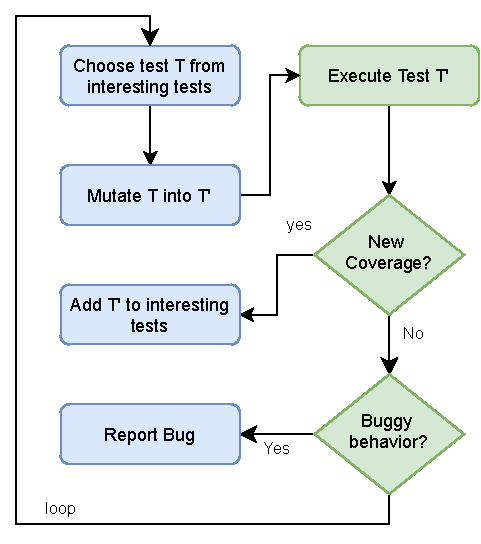
\includegraphics[width=0.7\linewidth]{mutation-fuzzing.pdf}
    \caption{Mutation-based fuzzing feedback loop. First start with a test, i.e.\ set of inputs, then mutate the test, execute it and evaluate how it effected the coverage. If the coverage changed, then the test is interesting else it isn't.}
\label{fig:mut-fuzz}
\end{figure}

Figure~\ref{fig:mut-fuzz} shows that, in mutation-based fuzzing, we start by defining well-formed inputs, a.k.a.\ seeds, and a coverage metric. 
We then mutate the seeds based on coverage feedback from a previous test in order to obtain new coverage results. 
The fuzzing stops once a target coverage percentage is reached.

We can then define a fuzzer with 3 elements:
\begin{itemize}
\item \textbf{Fuzz server}, which interfaces with the program under test (PUT) and resets it after each test.
\item \textbf{Instrumentation pass}, which is where the coverage-related modifications are made to the PUT.
\item \textbf{Fuzz engine}, which handles test mutation and coverage-feedback analysis.
\end{itemize}

\subsection{Chisel}
Our project focuses on RTL circuits designed in Chisel.
Chisel is a hardware construction language embedded in Scala~\cite{chisel:dac2012} that generates Verilog as a final output.
Chisel also generates code in an intermediate representation named \texttt{FIRRTL}\footnote{\url{https://github.com/freechipsproject/firrtl}}.(Flexible Intermediate Representation for RTL).
Chisel allows the user to describe RTL circuits in a high-level manner, using functional tools and libraries from Scala in order to minimize the amount of code needed to describe a circuit.
Since Chisel is a pure hardware \emph{construction} language, all valid Chisel code maps to synthesizable hardware.
Chisel also enables the verification engineer to use the full power of Scala and Java in a Chisel test-bench, thus making the verification more efficient.

\subsection{ChiselTest}
 
 There a many ways to test a Chisel design, but the most common are to write test-benches for the output Verilog.
 This is often done using either standard Verilog test-benches or more complex ones using SystemVerilog with UVM.
 
ChiselTest~\cite{chisel:tester2}, a nonsynthesizable testing framework for Chisel, offers another solution by allowing one to directly test the Chisel code in a usable and simple way.
ChiselTest works as a Scala library that allows the user to interface directly with the simulator with operations like \texttt{peek} (view the value of a wire), \texttt{poke} (write a value to a wire) and \texttt{step} (increment the clock).
%These tests are simple imperative Scala programs in which one line runs after the next.
In order to gain access to concurrency, the library also offers a \texttt{fork} method.

ChiselTest tries to enable best practices from software engineering by having lightweight syntax, allowing one to easily write small targeted unit tests.
Our project uses ChiselTest as a backend in order to access the simulator throughout the fuzzing cycle.

\subsection{ChiselVerify}

The presented fuzzer is part of the ChiselVerify project~\cite{verify:chisel:2020, dobis2021opensource}, available
at \url{https://github.com/chiselverify}.

\subsection{Simulators}

Chisel designs can be simulated by simulating the output Verilog or FIRRTL code.
The first one can be done using any available Verilog simulator.
Most of them, however, are proprietary and thus need expensive licenses in order to be used. 
The main open-source option is \texttt{verilator}~\cite{verilator}, which has a high compilation cost but has a good per-cycle efficiency.

The other option is to use a FIRRTL simulator, the main one being Treadle\footnote{\url{https://github.com/freechipsproject/treadle}}.
Treadle operates on FIRRTL and thus allows one to avoid generating Verliog code, which can vastly reduce the setup time for tests and efficiently run suites of many short tests.
ChiselTest and our solution work using Treadle as a simulator. 
%This allows us to have more control over the process by writing our own \texttt{FIRRTL} compiler passes, allowing for the gathering of specific coverage data.

%\todo{Check what ScalaCheck can offer.}

\section{Fuzzing with Chisel}
The main goal of this project is to enable the fuzzing of RTL circuits implemented in Chisel, while using functional coverage as a driving metric.
The mutation engine is taken form AFL using the Java Native Interface (JNI).
We will now present the fuzzer's current structure.

\subsection{Fuzzing algorithm}  
The fuzzer works in five main phases:  
\begin{itemize}
\item Interpret user-defined input files as bit-streams and load them into a queue.
\item Select the next file from said queue.
\item Mutate the file, using multiple passes of first deterministic then non-deterministic mutation techniques.  
\item Run the test and retrieve coverage results. 
\item Compare results to previous ones to determine if the new test was interesting or not. Add to the corpus of interesting tests if needed and repeat. 
\end{itemize}  

We will now discuss each of these points in detail.  
\subsection{Input file definition} 
Initial inputs are defined by the user and will be the base seeds of the test corpus.
This is done by defining a set of binary seed files that each contain a sequence of inputs for the DUT.

We define the input size as the sum of the bit length of all input signals of the DUT.
\begin{lstlisting}[captionpos=b,caption={Basic DUT with two 32 bit inputs, one 64 input, as well as a 32 bit output.},label={lst:dutexample},language=scala]
class DUT extends Module {
    val io = IO(new Bundle {
        val inA = Input(UInt(32.W))
        val inB = Input(UInt(32.W))
        val inC = Input(UInt(64.W))
        val out = Output(UInt(32.W))
 })}
\end{lstlisting}
For example, listing~\ref{lst:dutexample} has an input size of $32 + 32 + 64 = 128$ bits.
An input for this would thus be a 128 bit binary sequence, where the first 32 bits would be \texttt{inA}, second 32 bits \texttt{inB} and last 64 bits \texttt{inC}.
In order to define timing in our tests we can simply concatenate a second 128 bit sequence to the first one.
This second sequence will be fed to the DUT a single cycle later, thus creating a 2 cycle long test.
The total duration of a test is thus defined by the input file's bit-length divided by the input size of the DUT.

\subsection{Mutation engine}
Our fuzzer uses AFL's fuzzing engine, which works using multiple passes of both deterministic and non-deterministic mutation techniques.
The engine first starts by applying  the following series of deterministic mutation techniques:
\begin{itemize}
\item \textbf{Walking bit or byte flips}: Sequencially walk through each bit string row, either bit by bit or byte by byte, and flip either 1, 2 or 4 bits or bytes per pass.
\item \textbf{Simple arithmetics}: Add or subtract values to the bit string. This is usually done by doing multiple incrementation or decrementations at different bytes throughout the string.
\item \textbf{Known integers}: Use preset interesting integer values (like 0x7F or 0xFF) to replace bytes throughout the string.
\end{itemize}
After using the above deterministic mutation methods, the engine moves on to non-deterministic mutations like stacked tweaks or test case splicing, which are covered in detail in AFL's documentation~\cite{afl:fuzzingtechniques}.
%\todo{Talk about AFL's mutation techniques.}
\subsection{Result definition and comparison}
Throughout the fuzzing cycle, data is accumulated in the form of pairs containing both the test's input bit string and the values of the hits that they generated for each \texttt{cover} construct defined in the verification plan~\cite{dobis2021opensource}.
These \texttt{(Test, hit values)} pairs are then used to identify whether or not an input bit string was interesting.
An interesting input is defined as any input that generated a set of hit values that is not a subset of an existing interesting result.
These results also contain a total obtained functional coverage, which is the average coverage over all defined \texttt{cover} constructs in the verification plan.
The coverage allows us to know when to stop fuzzing and output a final result.

%\todo{Talk about how to define a result and how to compare two results together and remove obsolete entries. Result = (Test, values hit) and \texttt{res1} $\subseteq$ \texttt{res2} $\Leftrightarrow$  \texttt{res1}'s values have also been hit in \texttt{res2}}

\subsection{Fuzzer interface}
The interface for our fuzzer is defined as follows:
\begin{lstlisting}[captionpos=b,caption={Interface for the ChiselVerify fuzzer. It takes as parameter a \texttt{dut} and \texttt{chiselverify.coverage.CoverageReporter}, which is the verification plan used to define the functional coverage that will drive the fuzzing. It also takes in a target coverage percentage between 0 and 100, which defaults to 100, and a timeout which is set by default to 1'000'000 inputs. The second set of parameters are a result output file name, where all of the interesting tests and their resulting hit values will be written, as well as a variable number of file paths, which will be used as seeds for the mutation engine. },label={lst:dutexample},language=scala]
object Fuzzer {
    def apply[T <: MultiIOModule](
        dut: T, 
        funCov: CoverageReporter, 
        target : Int = 100,
        timeout : BigInt = BigInt(1000000))
        (result: String
        seeds: String*) : Int
}
\end{lstlisting}
The fuzzer itself will run either until the target coverage or the timeout is reached. The value returned is the final coverage percentage attained during the fuzzing.

\section{First Experiments}
\label{sec:eval}
%
%\martin{Can we make a quick and dirty (dumb) fuzzing with Leros?}
%\martin{Hopefully not just the ALU, maybe the whole processor}

Although this is a work-in-progress report, we have started with an evaluation.

For our evaluation, we used an ALU with an accumulator from the Leros processor~\cite{leros:arcs2019}
as our device-under-test (DUT).
The example is simple, but has a combinational part and state in a register, being
a non-trivial circuit for testing.

We start by creating a verification plan using functional coverage tools from ChiselVerify.
\begin{lstlisting}[captionpos=b,caption={Simple verification plan for the leros ALU. Since this is still a work-in-progress, the verification plan is simple and only contains basic cover points. The functional coverage code is also abridged since it is not our main focus in this paper.},label={lst:lerosfuncov},language=scala]
val cr = new CoverageReporter(dut)
cr.register(
    cover("op", dut.input.op)(
        bin("nop", 0 to 0),
        //[...] Bins for each operation
        bin("shr", 7 to 7)),
    cover("din", dut.input.din)(
        bin("0xF", 0 to 0xF),
        //[...] Cover all ranges
        bin("0xFFFF", 0xFFF to 0xFFFF)),
    cover("accu", dut.output.accu)(
        //[...] Same as din
    cover("ena", dut.input.ena)(
        bin("disabled", 0 to 0),
        bin("enabled", 1 to 1)))
\end{lstlisting}
Listing~\ref{lst:lerosfuncov} shows a verification plan that covers all possible values for the ALU's inputs.
Once the verification plan is defined, we create a binary input file.
To do that, we write a series of simple operations for the ALU to perform and encode them in a binary format stored in seed files.
\begin{lstlisting}[captionpos=b,caption={Basic ALU operations; dut.io.op is 3 bits wide and din is 8 bits wide. Each binary input in the example is separated with a whitespace for clarity.},label={lst:binops},language=C]
//32 + 25, done by loading 32 and adding 25 
//op = 6; din = 0x20; 
//op = 1; din = 0x19;
//op = 0; din = 0;

//Binary input stream:
110 00100000 001 00011001 000 00000000
\end{lstlisting}
Listing~\ref{lst:binops} is a basic binary seed saved in a file named \texttt{seed.bin}.
All that is left is to run the fuzzer on our design with the given seed.
\begin{lstlisting}[captionpos=b,caption={Call to the fuzzer using the setup previously described.},label={lst:fuzzcall},language=scala]
Fuzzer(dut, cr)("output.txt", "seed.bin")
\end{lstlisting}

\todo{Obtain max coverage results with basic seed and discuss.}
We see that we need more seeds in order to obtain better maximum coverage results. 
The reason for that is that with a single seed, the initial corpus will always be a continuous mutation of the same test and it is thus more likely to obtain invalid inputs.
Adding more input seeds covering all possible operations increased the maximum coverage result to \todo{insert percentage} using the same timeout.
The execution time is slower than RFuzz with the same seeds, since they have the benefit of FPGA acceleration.
However, our coverage target is attained using \todo{get exact iterations} iterations where RFuzz requires \todo{get iterations} iterations to reach the same coverage goal.
This shows that the use of functional coverage, instead of the edge coverage used in RFuzz and AFL, will lead to less iterations required to obtain a satisfactory coverage percentage, since functional coverage gives the fuzzer more information about the internals of the DUT it is testing.

\subsection{The Road Ahead}
Since this project is still a work-in-progress, the evaluation has still only been done with simple designs, such as an ALU.
The discussed fuzzing techniques can also be applied to processors where instead of input sequences, a coherent program is generated and mutated to maximize the functional coverage of the circuit. 
This requires a constrained random program generator which can be interfaced by a fuzzer and used as an alternative mutation engine.
This will result in more efficient processor fuzzing, since it will only generate legal instructions. 

As a part of the ChiselVerify project, we have started to develop a constrained random assembly program generator with the goal of combining it with the developed fuzzer to ameliorate processor mutation-based fuzzing in Chisel.
%=======
%\subsection{Constrained Random Program Generation}
%
%The discussed fuzzing techniques can not only be applied to verify classical digital circuits but also 
%processors where instead of input sequences, a program is generated and mutated to maximize the 
%functional coverage of the circuit. This requires a constraint random program generator which can 
%be interfaced by a fuzz engine and a coverage collector which can extract coverage data from the 
%generated program. 
%
%As a part of the chiselverify framework, we have started to develop a constraint random assembly 
%program generator with the long term goal of combining it with the developed fuzz engine to give 
%access to mutation based fuzzing in chisel/scala for processor verification.
%
%There are existing solutions for constrained random program generation, notably the open-source 
%RISC-V DV framework \cite{riscvdv} built using python and SystemVerilog. An implementation in 
%the chisel/scala framework will have the advantage of keeping all communication between the 
%constraint random program generator, the fuzz engine and the coverage collector in the same 
%language. Furthermore, our implementation will not limit itself to one ISA but will provide 
%a general infrastructure for RISC architectures and ISA definitions will be kept as libraries.

There are existing solutions for constrained random program generation, notably the open-source RISC-V DV framework \cite{riscvdv} built using python and SystemVerilog. 
An implementation in scala will have the advantage of keeping all internal communications in the same language. 
Our implementation will not limit itself to one ISA but will provide a general infrastructure for RISC architectures and ISA definitions will be kept as libraries.

\subsection{Source Access}

The library for this project is available on GitHub:\\ \url{https://github.com/chiselverify}.
We plan also to regularly publish it on Maven.
%\todo{Publish it and provide the info here.}
\section{Conclusion}
\label{sec:conclusion}

This work-in-progress paper is an initial sketch of supporting testing and verification
of digital designs described in Chisel with fuzzing. 
Inspired by ideas introduced by the software world, we presented a version of mutation-based fuzzing driven by a hardware-oriented coverage metric.
This allows a fuzzer generate tests that are more interesting for RTL designs and give the user more control over its behavior. 
Our plans are now to continue our work by enabling constrained generation of programs in order to test processor designs, thus orienting fuzzing towards RTL design verification.
%
%\subsection*{Acknowledgment}
%
%\martin{Do we have something here?}

\bibliographystyle{plain}
% Please do not add any references to msbib.bib.
% They get lost when I 'generate' is again (see Makefile)
\bibliography{../chisel-uvm,../msbib}

\end{document}